% !TeX root = ../main.tex
% Add the above to each chapter to make compiling the PDF easier in some editors.
\chapter{Methodology}\label{chapter:method}
We aim to solve two problems: First the raw dataset being available centrally itself and second the risk of inference attacks. Most research is based on datasets that span only over a few days or weeks. When collecting location data over months, the chance of successful inference attack increases in all cases with more data available.

In order to address the problem and test our hypothesis, we propose a framework in which we collect and locally aggregate location data on end user devices (smartphones) throug an application designed for this purpose. The raw data will stay on each device and will only be used to serve aggregation requests. The aggregation requests have to be defined upfront. An example is the determination of the average steps per day by each user. An incoming aggregation request might look like
\begin{verbatim}
{
	"start": "2019-05-30",
	"end": "2019-06-02",
	"type": "steps",
	"n" : 3,
	"value": 2000,
	"valueList": []
}
\end{verbatim}
And the data contained in the outgoing response after processing the request might look like
\begin{verbatim}
{
	"n" : 4,
	"value": 2500,
	"valueList": []
}
\end{verbatim}
 In order to protect the user's privacy and completely shield the raw data from the server, it would be necessary to pass the request via P2P from one device to another until the last device finally sends the results to the server. P2P on mobile phones though is hardly possible. On the other hand, if the server is used to pass an aggreation request from one device to another, it could read the data and compute the respective user's input from the difference. We propose to use encryption in order to hinder the server from reading the data. On installation of the application on a smartphone, a public-private key-pair is generated and every installed application registers at the server with this public key. The corresponding private key is stored locally. On start of an aggregation request, not only the first user but also the following user who should deal with the aggregation request is determmined and the public key of the next user is passed along with the aggregation request. When one end user device needs to send the processed aggregation request to the next phone, it encrypts the data using the provided public key of the next user in the standard hybrid encryption\footnote{In hybrid encryption as used in SSL, the message itself is encrypted with a synchronous key while this key itself is encrypted using the public key} approach leveraging the benefits of synchronous keys. This way the next phone in the aggregation chain will be able to decrypt the request and process the data while the server is unable to read the data until the aggregation request is finally send in plain text for publishing to the server. This process is depicted in figure XX.

 The aggregated results are available only to our research team in order to protect the research participants privacy in case there is a privacy risk we have not thought of but the setting allows for them being available to the public. The aggregation requsts themselves are controlled by our research team and inserted on a daily basis.

 \subsection{Aggregation schemes}\lebel{aggregation-schemes}
 We found two types of aggregation requests to be of interest. First, the evalulation of mean values and second, the evaluation of more advanced statistical values such as median or other percentiles and distribution. The latter includes the possibility to calculate the former. Nevertheless, we want to test all research questions independently.
 We found the following aggregations to be especially of interest:
 \begin{enumerate}
 	\item Computing the average number of steps walked across all users participating in the request. (e.g. to calculate how many people reach the 10.000 steps per day\footnote{It has to be evaluated, which percentage of steps are registered because the phone will not always be on the person}.)
	\item Computing the average time spent walking, running, in a vehicle or on a bicycle\footnote{https://developers.google.com/android/reference/com/google/android/gms/location/DetectedActivity}.
	\item Computing how many people respectively which share of people combine using a bicycle with using a vehicle such as public transport or a car in one trajectory.
	\item How much time do people stay at work.
	\item How long do people travel to work.
	\item Where did many participants spend a significant amount of time on a certain day? (Event recognition)
	\item What percentage of whole travelling time do people spend on their bike, car, ...
	\item What is the average speed on roads.

	\item Collecting a list of the average number of steps walked by each participant during the timespan.
	\item Collecting a list of the duration of all registered activities.

	\item collecting a list of all trajectories registered by the users' phones.
 \end{enumerate}
 For all these and more aggregations, always both, the mean value and if possible, a complete list of values to compute other statistical figures are of interest.

 \subsection{Narrowing the area of the aggregation request}

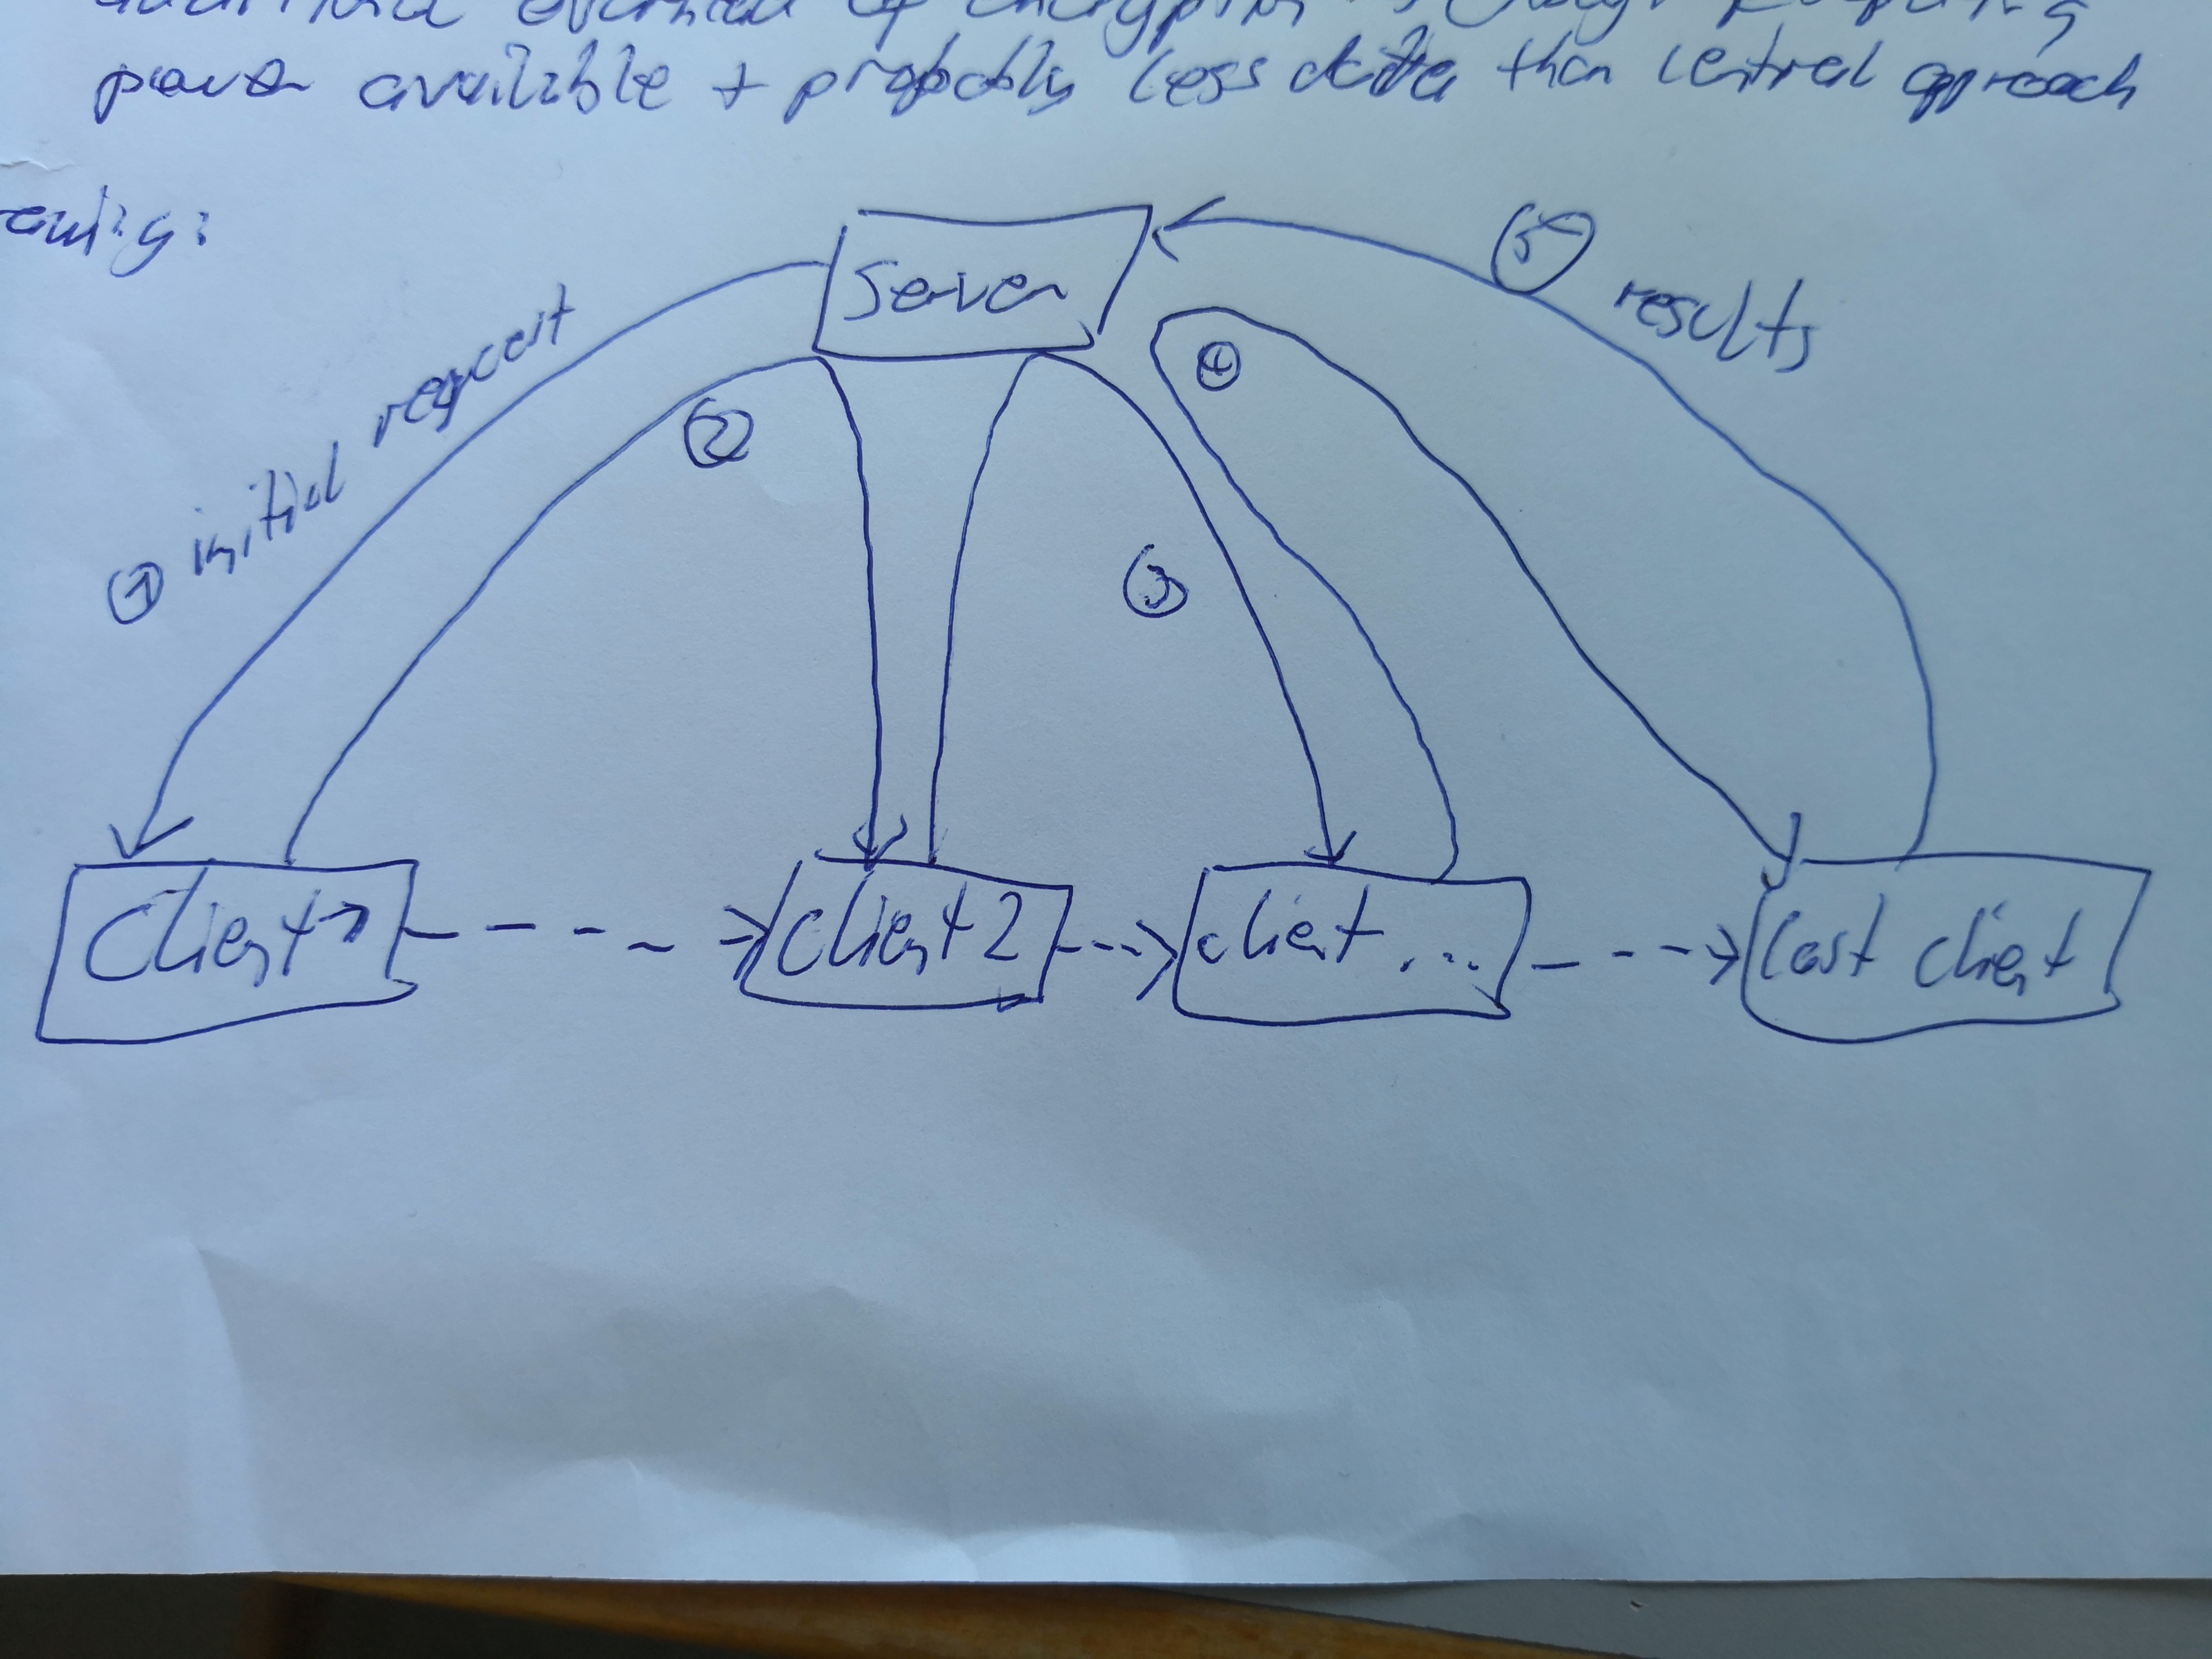
\includegraphics[width=\textwidth]{data/concept.jpg}

